\documentclass[12pt,a4paper,spanish]{article} 

\usepackage{graphicx} %option specific for pdfLatex compilation
\usepackage{makeidx}
\usepackage{lscape}
\usepackage{framed}
\usepackage{listings}
\usepackage[spanish]{babel}
\usepackage[utf8]{inputenc} 
\usepackage{indentfirst}
\usepackage{varwidth}
\usepackage[margin=1in]{geometry}


\begin{document}
\begin{titlepage}
\begin{center}

% Upper part of the page. The '~' is needed because \\
% only works if a paragraph has started.

\textsc{\LARGE \textbf{Universidad de Buenos Aires}}\\%[1cm]
\vfill
\textsc{\LARGE \textbf{Técnicas de Programación Concurrente I }}\\%[0.5cm]
\vfill
\textsc{\LARGE \textbf{(75.59)}}\\%[0.5cm]
\vfill
% Title
%\HRule \\[0.4cm]
\vfill
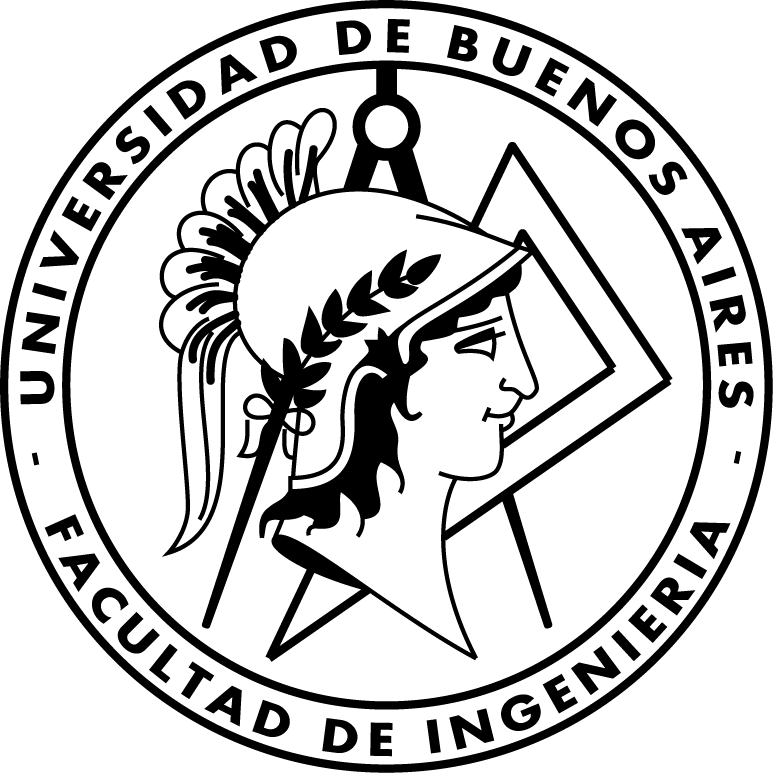
\includegraphics[scale=1.25]{./logo.png}~\\[2cm]
%\HRule \\[1.5cm]
{ \huge \bfseries Trabajo Práctico Nº 1}\\%[0.25cm]
\vfill
%{ \huge \bfseries Grupo 8}\\%[0.25cm]
%\vfill
{\Large
\begin{tabular}{|c|c|c|}
\hline
Nombre y apellido & Padrón & Mail \\
\hline
Florencia Bosch & 91867 & florb\_128@hotmail.com \\
\hline
Javier Choque & 92079 & javierchoque21@gmail.com \\
\hline
Pablo Musumeci & 92165 & pablomusumeci@yahoo.com.ar\\
\hline
\end{tabular}
}
\vfill

% Bottom of the page
{\large \today}

\end{center}
\end{titlepage}

\newpage
\tableofcontents
\newpage
\section{Hipótesis}

A continuación se presentan los supuestos que consideramos a la hora de desarollar el 
trabajo práctico.


\begin{itemize}
	\item Consideramos que cuando un auto es enviado a la salida por el Jefe de Estación,
	el mismo sale del sistema de manera instantánea, sin tener que hacer una cola
	para salir de la estación.

	\item El administrador no tiene prioridad sobre los empleados al momento de consultar
	el saldo en la caja, y debido a esto, cuando desea hacerlo debe aguardar su turno para
	trabajar de manera exclusiva con la caja, al igual que cualquier empleado.

	 \item Con la finalidad de que la simulación represente una situación real, la cantidad
	 de surtidores y empleados que tiene la estación al momento de comenzar la misma debe ser 
	 mayor a 0.
\end{itemize}

\newpage

\section{Diseño}
	\subsection{Proceso Principal}

		Es el encargado de lanzar los procesos que componen la simulación, inicializar los recursos
		compartidos como semáforos y memorias compartidas.

		También se encarga de, cuando el usuario decide finalizar la simulación, enviar las señales
		apropiadas para que dichos procesos cesen el uso de los recursos. Luego, espera a la finalización
		de dichos procesos hijos, para finalizar la simulación.

	\subsection{Generador de Autos}
		
		Este proceso es el encargado de crear los autos que llegan a la estación. Para
		dicho propósito, genera autos en intervalos de tiempo especificado en el archivo de configuración. 
		Cada auto está representado por un ID y una cantidad de dinero que va a gastar en la estación.

		El Generador de Autos interactúa con el Jefe de Estación, y dicha interacción se puede
		asemejar al problema \textbf{Producer - Consumer}, debido a que el Generador produce
		los autos que el Jefe de Estación va a recibir. 

		La comunicación entre el Generador de Autos y el jefe de Estación se realiza por medio de un
		FIFO.


	\subsection{Jefe de Estación}
		Este proceso se encarga de recibir los autos nuevos que van llegando a la estación. 
		En este caso, el Jefe de Estación es el \textbf{consumer} de información.

		Una vez que logró extraer un automóvil del buffer exitosamente, debe asignarle 
		un empleado al auto recibido, en caso de que exista algun empleado disponible 
		en ese mismo instante, caso contrario, deberá redirigir el mismo hacia la salida.
		
		El jede de estación, lee un variable que se encuentra en memoria compartida, la cual
		representa el número de empleados disponibles en ese momento. Para acceder a dicha variable,
		deberá pedir acceso a un semáforo que restringe su uso de manera exclusiva.
		En el caso de exista algún empleado libre (lo cual se deduce de que el valor de dicha variable
		es mayor a cero), escribe el automóvil recibido por parte del generador en un FIFO.


	\subsection{Empleado}
	
		Este proceso representa el accionar de un empleado cuando atiende un auto. Los empleados piden acceso
		de manera exclusiva a FIFO en el que el jefe de estación escribirá los autos, de manera que no se
		atienda a un auto más de una vez por diferentes empleados. El acceso al FIFO por parte de los empleados,
		se encuentra controlado por un semáforo. 

		Una vez que un empleado recibe un auto, modifica la variable que lleva la cuenta de los empleados libres, 
		disminuyendo en uno su valor. Una vez que el empleado tiene el automóvil en su poder, se dirige hacia los
		surtidores, esperando en un semáforo que representa la cantidad de surtidores disponibles. 

		El tiempo de atención del automóvil se calcula a partir del dinero que lleva el mismo. Dicho tiempo no es
		proporcional al dinero que el automóvil dispone. Luego de la espera, libera el surtidor utilizado y se dirige
		a la caja para depositar el monto que el mismo llevaba. La caja, es implementada como una variable del tipo entero
		en memoria compartida, que debe accederse de a un proceso a la vez por medio de un semáforo.

		Cuando se finaliza la atención del automóvil, el empleado incrementa la variable que representa la cantidad
		de empleados libres, y vuelve a pedir acceso al FIFO en la espera de un nuevo cliente
	
	\subsection{Administrador}
	
	El proceso administrador tiene la facultad de consultar el valor guardado en la caja. Puede hacerlo en cualquier momento, y su consulta sobre la caja esta controlada de la misma forma que el empleado. La diferencia con el empleado es que el Administrador no espera a un auto, sino que puede consultar en cualquier momento. En nuestra implementación, 
	el administrador consulta la caja de manera periódica, siendo configurable el período de espera entre cada consulta.

\subsection{Casos de uso}

\begin{itemize}
	\item Inicar simulación: El actor que dispara este caso de uso es el usuario
	que desea iniciar la simulación. Para iniciar el programa se debe ejecutar el
	proceso \texttt{procesoPrincipal}, el cual se encarga de
	lanzar a los otros procesos involucrados en el funcionamiento de la simulación.

	Es necesario que la ejecución del proceso principal se realize con los parámetros
	que indican la cantidad de empleados (por medio de la expresión \texttt{-e} o \texttt{--empleados})
	y la cantidad de surtidores (\texttt{-s} o \texttt{--surtidores})que que tendrá la
	estación de servicio.

	Ejemplo:

	\texttt{./procesoPrincipal -e 5 -s 7}

	\item Finalizar la simulación: El proceso principal se quedará esperando por el 
	ingreso de un caracter cualquiera, como orden para finalizar todos los procesos
	que componen la simulación.

\end{itemize}


	\section{Diagrama esquemático de interacciones}
	
	Ver figura \ref{diagrama}

\begin{figure}
\label{diagrama}
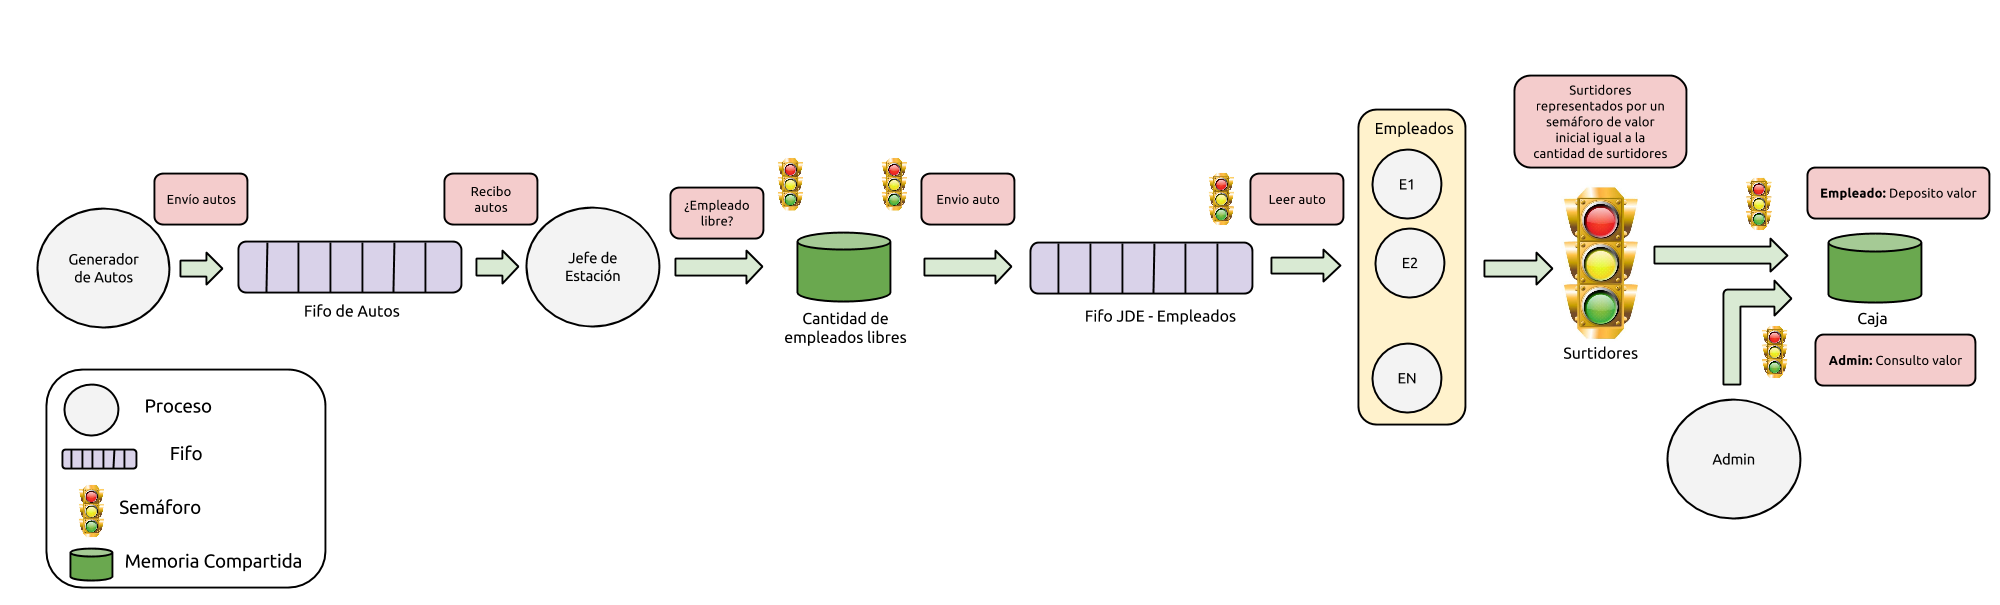
\includegraphics[angle=90, scale = 0.34]{esquema.png}
\centering
\caption{Diagrama esquemático de interacciones}
\end{figure}

\newpage
	\section{Datos compartidos entre procesos}
	
	\begin{itemize}
	
	\item Generador de Autos - Jefe de Estación:
		\begin{itemize}
			\item Fifo \texttt{files/generador.jde} para envío de los autos
		\end{itemize}
	
	\item Jefe de Estación - Empleado:
	\begin{itemize}
		\item Fifo \texttt{files/jde.empleado} para envío de los autos
		\item Memoria compartida con la cantidad de empleados disponibles
		\item Semáforo para controlar acceso a la memoria compartida.
		\item Semáforo para controlar acceso al Fifo, por parte del empleado (lector).
	\end{itemize}

	\item Empleado (surtidores):
	\begin{itemize}
		\item Semáforo \texttt{files/semaforo.surtidores} que representa la 
		cantidad de surtidores libres, y controla el acceso a los mismos.
	\end{itemize}

	\item Empleado (caja):
	\begin{itemize}
		\item Memoria compartida que representa la caja
		\item Semáforo que controla el acceso a la caja
	\end{itemize}

	\item Administrador (caja):
	\begin{itemize}
		\item Memoria compartida que representa la caja
		\item Semáforo que controla el acceso a la caja
	\end{itemize}

	\end{itemize}
	\newpage
	\section{Diagrama de estados del proceso Jefe De Estación}

	\begin{figure}[h]
	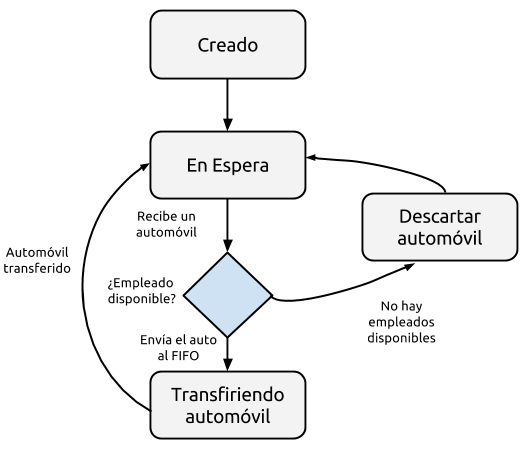
\includegraphics[scale=0.75]{FSM_JDE.png}
	\centering
	% https://docs.google.com/drawings/d/1fSqCpKnnYxksGUfpufRSJbsfxkYRRuSEGUDkyJf5Sf0/edit?usp=sharing
	\caption{FSM del Jefe de Estación}
	\end{figure}

	\newpage
	\section{Diagramas de clases}
	\subsection{Generador de automóviles y Jefe de estación}
	\begin{figure}[h]
	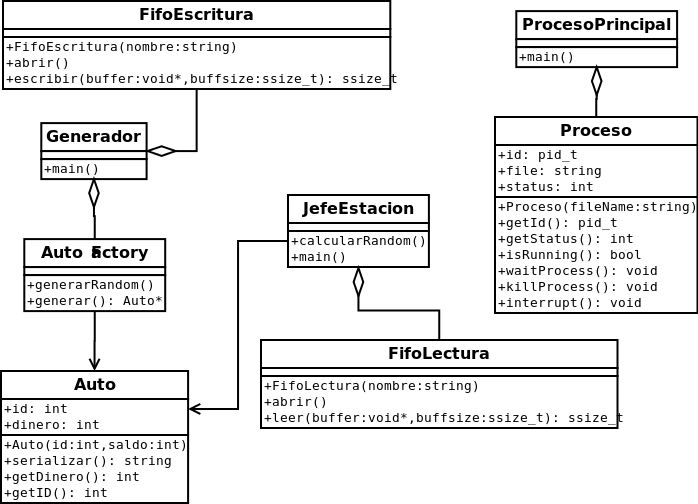
\includegraphics[scale=0.60, angle=90]{GeneradorJde.png}
	\centering
	\end{figure}

	\newpage		
	\subsection{Jefe de estación y empleado}
	\begin{figure}[h]
	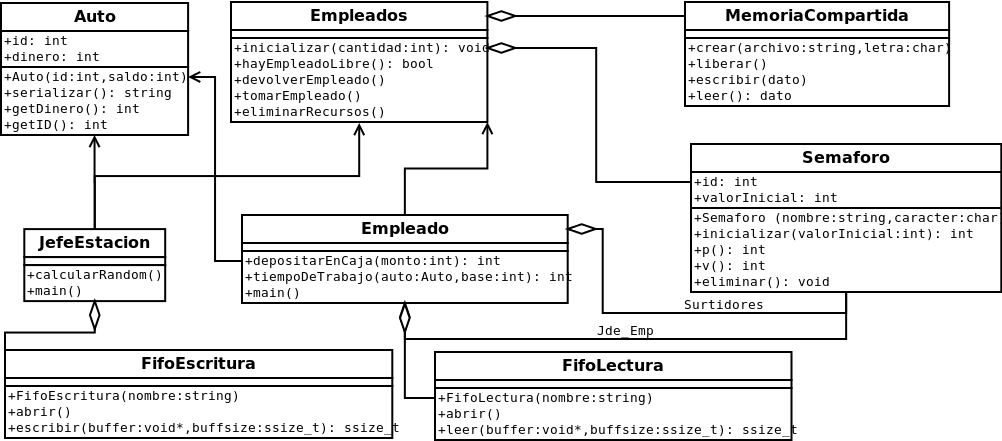
\includegraphics[scale=0.50, angle=90]{JDE_Empleado.png}
	\centering
	\end{figure}

	\newpage	
	\subsection{Empleados, administrador y acceso a la caja}
	\begin{figure}[h]
	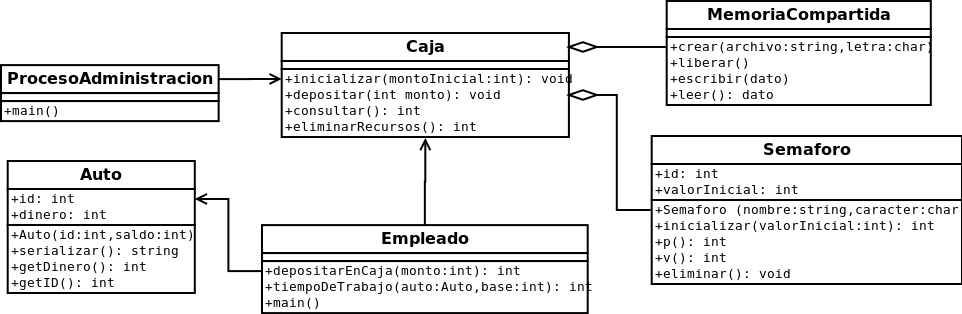
\includegraphics[scale=0.50, angle=90]{AccesoCaja.png}
	\centering
	\end{figure}

	\newpage

	\section{Parte 2}

	\subsection{Diseño}

	En esta sección vamos a detallar las modificaciones realizadas para cumplir con
	los requerimientos presentes en el enunciado.

	\subsubsection{Proceso Caja}

	Introducimos en el diseño de la solución un nuevo proceso para lidiar con el siguiente requerimiento:

	\begin{framed}
	El administrador deberá tener prioridad sobre los empleados al momento de utilizar la caja.
	\end{framed}

	El \emph{Proceso Caja} es el encargado de controlar el acceso a la misma, la cual ha dejado de estar en memoria
	compartida (como era el caso en el trabajo práctico 1) para pasar a ser una variable entera que reside en la
	memoria de dicho proceso.
	Esto se debe a que, para satisfacer la restricción impuesta, ya que tenemos un proceso que controla el acceso,
	y es el único que va a interactuar de manera directa con la caja, dejo de ser necesario que la misma se encuentre
	en memoria compartida.

	Los procesos \emph{empleado} y \emph{administrador} se comunicaran con el \emph{Proceso Caja} por medio de dos colas de mensajes, envíando peticiones al \emph{Proceso Caja}, dichas peticiones están compuestas por los siguientes valores:

	\begin{description}
		\item[mtype] Representa la prioridad del proceso que realiza la petición.
		\item[id] Identificador unívoco del procesoque realiza la petición.
		\item[dinero] Dinero que se desea depositar en la caja.
	\end{description}

	\begin{center}
		\begin{varwidth}{0.5\textwidth}
			\begin{lstlisting}[frame=single, language=C, caption={Peticiones encoladas}]
			
typedef struct st_peticion {
	long mtype;
	pid_t id;
	int dinero;
} st_peticion;
			\end{lstlisting}
		\end{varwidth}
	\end{center}
	Con dicha interfaz, se resuelven las 2 peticiones posibles, debido a que, si el \emph{administrador}
	desea consultar el valor de la caja, solo debe enviar la estructura que se muestra a continuación con el
	atributo dinero en cero.

	Una vez realizada la petición por un proceso, el mismo debe esperar la llegada de un mensaje que le
	de confirme su depósito. Dicha espera la realiza leyendo en la cola de recepción, y la misma representa
	el tiempo que el empleado esta haciendo cola para depositar el valor recibido.

	Como contrapartida, el \emph{administrador}, quien tiene una prioridad mayor a los empleados, realiza su
	petición y espera la resputa al igual que los empleados, y en dicha respuesta recibe el saldo que se 
	encuentra en la caja.

	\subsubsection{Distinción entre surtidores}

	En la segunda parte del trábajo práctico, debemos realizar un cambio respecto a la asignación de surtidores,
	ya que en la primer entrega no era necesario distinguir cual se estaba utilizando. 
	
	\begin{framed}
	Se deberá poder tracear en el log de la simulación que empleado atendió a que auto y que surtidor
	utilizó al hacerlo.
	\end{framed}

	Para la primer entrega, los surtidores estaban realizados como un semáforo de valor igual a la cantidad
	de semáforos requerida para la simulación. Dicha implementación nos permitía controlar que no se 
	utilizen m`as surtidores de los disponibles en determinado momento, pero no nos dejaba idenfiticar
	cual de ellos se estaba utilizando.

	La forma elegida para cumplir con la especificación solicitada, fue agregar una cola en donde se guardan
	los surtidores, en donde cada uno esta asociado con un identificador unívoco. Los empleados desencolan
	un surtidor, trabajan y cuando han finalizado su labor vuelven a encolar el surtidor utilizado. De esta manera, si un empleado quiere trabajar y no un surtidor libre que pueda utilizar, se quedar`a esperando en la cola hasta que uno se libere.

	\subsubsection{Comunicación Generador - Jefe de estación}

	A continuación detallemos otra de las modificaciones realizadas, esta vez para cumplir con el siguiente requerimiento:
	
	\begin{framed}
	La estación de servicio cuenta con dos tipos de clientes: regulares y VIP
	\end{framed}

	En le trabajo práctico 1, el envío de autos entre el proceso \emph{Generador de Autos} y el proceso \emph{Jefe de Estación}
	se llevaba a cabo por medio de un FIFO. 

	Se reemplazo dicho medio de comunicación por una cola de mensajes en donde el Generador encola los autos que va generando 
	(con cierta probabilidad de generar un cliente VIP) y el Jefe va desencolando los mismos por orden de prioridad (y ante la misma prioridad desencola el primer elemento de la cola que cumpla la condición, ergo, el que hace más tiempo se encuentra 
	esperando en la misma).

	Los autos guardan sus datos dentro de un struct con el método \texttt{getStruct()} y el proceso generador de autos lo encola.
	Luego, el proceso Jefe de Estación desencola el struct e hidrata el auto con el método \texttt{fromStruct(const st\_auto\& structAuto)}.

\begin{center}
		\begin{varwidth}{0.5\textwidth}
			\begin{lstlisting}[frame=single, language=C, caption={Autos encoladas}]
	typedef struct st_auto {
	long mtype;
	int id;	
	int dinero;
} st_auto;
		\end{lstlisting}
	\end{varwidth}
\end{center}
	\newpage
	\subsection{Diagrama esquemático de interacciones}
	
	\begin{figure}[h]
	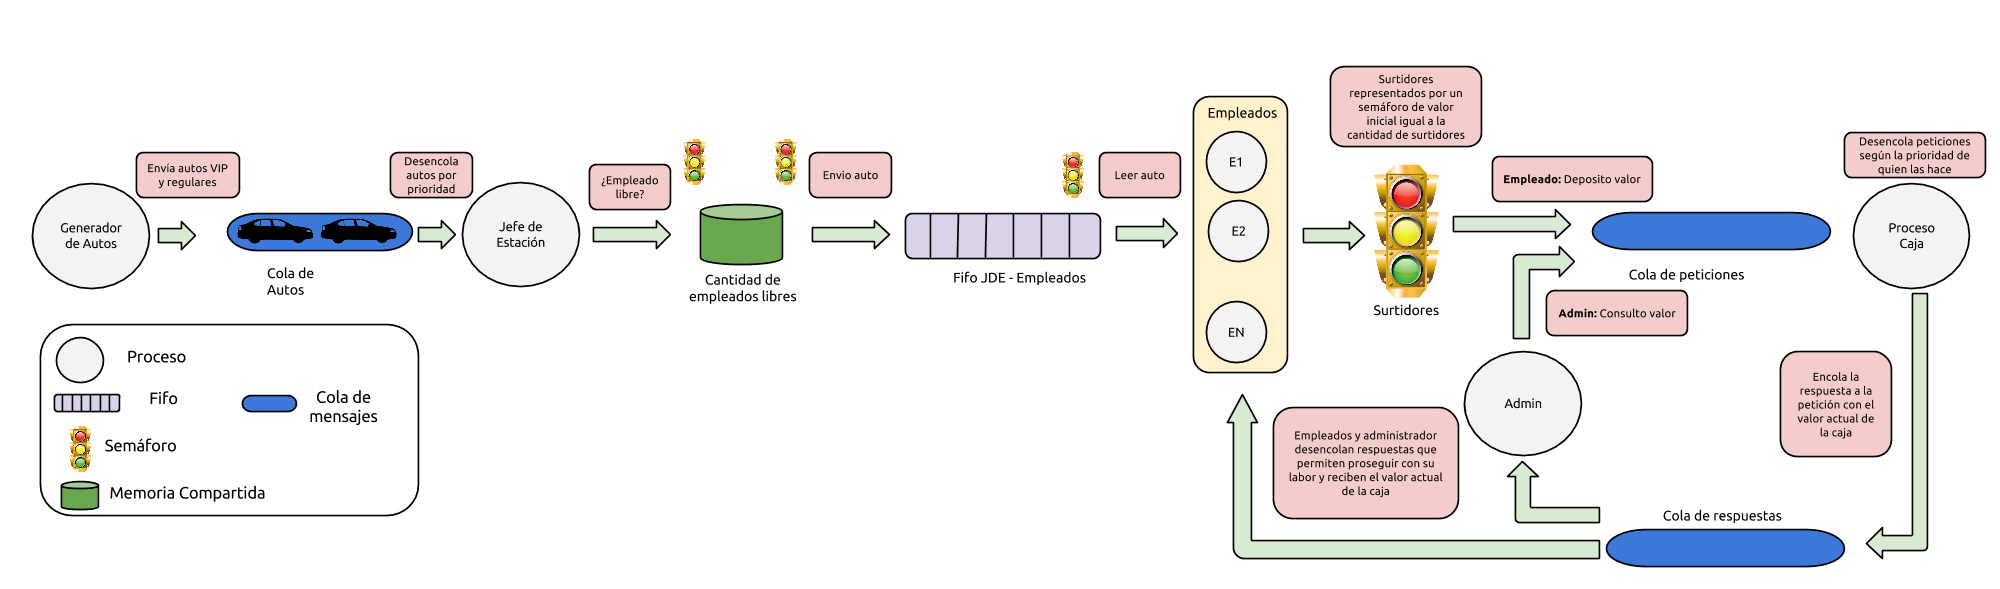
\includegraphics[angle=90, scale = 0.27]{esquema_2.png}
	\centering
	\end{figure}

	\newpage
	\subsection{Casos de uso}

	\begin{figure}[h]
	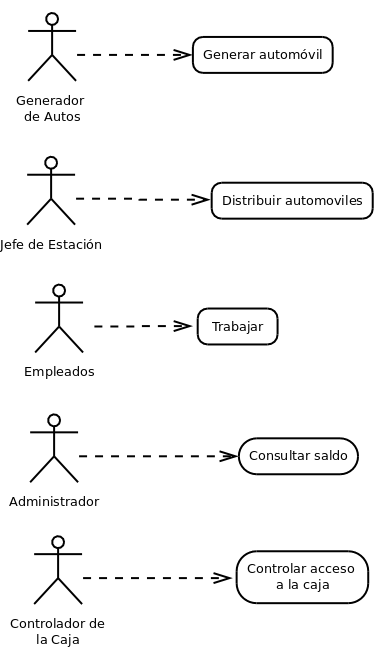
\includegraphics[scale=0.50]{casos_de_uso.png}
	\centering
	\end{figure}

    \begin{tabular}{|p{4cm}|p{12cm}|}
    \hline
    \textbf{Caso de uso:} & Generar auto \\
    \hline
    \textbf{Descripcion:} &  Crea el automovil que se dirige a la estacion\\
    \hline
    \textbf{Actores participantes:} & Generador de autos  \\
    \hline
 
    \textbf{Pre-condiciones:} &  El proceso principal inicializo los recursos utilizados\\
    \hline
    \hline
    \textbf{Flujos:} &\\
    \hline
	\textbf{Flujo Principal:} &\\ 

	\hline
	1 & El generador utiliza un numero aleatorio para determinar si el auto creado sera VIP o regular\\
    \hline
	2 & El generador asigna un ID autoincremental al automovil creado\\
    \hline
	3 & El generador crea un struct con los datos del automovil creado\\
    \hline
	4 & El generador escribe en la cola el struct mencionado anteriomente\\
    \hline
	5 & El generador duerme un tiempo constante (configurable) antes de enviar otro automovil\\
    \hline
    \hline
	\textbf{Flujos de excepción:} & Se recibio una señal que cambia la condicion del while que ejecuta el proceso. En la proxima iteracion se saldra del ciclo y terminara el proceso.\\
    \hline
	\textbf{Post-condiciones:} & Se encolo un automovil en la cola que comparten el generador y el jefe de estacion\\
	\hline
	\end{tabular}

	\newpage

	\begin{tabular}{|p{4cm}|p{12cm}|}
    \hline
    \textbf{Caso de uso:} & Distribuir automoviles \\
    \hline
    \textbf{Descripcion:} &  Despacha automoviles hacia los empleados o la salida\\
    \hline
    \textbf{Actores participantes:} & Jefe de estacion  \\
    \hline
 
    \textbf{Pre-condiciones:} &  El proceso principal inicializo los recursos utilizados. Existe 
    al menos un auto encolado por el generador.\\
    \hline
    \hline
    \textbf{Flujos:} &\\
    \hline
	\textbf{Flujo Principal:} &\\ 

	\hline
	1 & El JDE desencola un auto\\
	\hline
	2 & Consulta la variable en memoria compartida que tiene la cantidad de empleados disponibles\\
	\hline
	3 & El generador crea un struct con los datos del automovil creado\\
	\hline
	4 & Existe un empleado disponible
		\begin{itemize}
			\item Enviar automovil por el FIFO entre JDE y empleados 
		\end{itemize}
		\\
	\hline
	5 & No existe un empleado disponible
		\begin{itemize}
			\item Se descarta el automovil
		\end{itemize}
		\\
	\hline
	\hline
	\textbf{Flujos de excepción:} & Se recibio una señal que cambia la condicion del while que ejecuta el proceso. En la proxima iteracion se saldra del ciclo y terminara el proceso.\\
    \hline

    \hline
	\textbf{Post-condiciones:} & Se desencolo un automovil de la cola compartida entre el generador y el JDE.\\
	\hline
	\end{tabular}

	\newpage

	\begin{tabular}{|p{4cm}|p{12cm}|}
    \hline
    \textbf{Caso de uso:} & Empleado trabajando \\
    \hline
    \textbf{Descripcion:} &  Ciclo de trabajo del empleado\\
    \hline
    \textbf{Actores participantes:} & Empleado\\
    \hline
 
    \textbf{Pre-condiciones:} &  El proceso principal inicializo los recursos utilizados. El empleado tiene un auto leido del FIFO compartido con el JDE\\
    \hline
    \hline
    \textbf{Flujos:} &\\
    \hline
	\textbf{Flujo Principal:} &\\ 

	\hline
	1 & El empleado decrementa la variable que representa la cantidad de empleados disponibles\\
	\hline
	2 & El empleado se queda leyendo de la cola de surtidores hasta poder conseguir uno\\
	\hline
	3 & Calcula el tiempo a trabajar a partir del dinero que tiene el automovil\\
	\hline
	4 & Duerme el tiempo calculado\\
	\hline
	4 & Envia una solicitud para depositar el dinero en la caja (escribiendo en la cola) \\
	\hline
	5 & Lee en la cola hasta recibir la respuesta de que su solicitud fue exitosa (y asi simula la espera en la caja)\\
	\hline
	6 & Encola el struct que representa al surtidor utilizado, dejandolo libre para que lo use otro empleado\\
	\hline
	7 & Aumenta la cantidad de empleados disponibles\\
	\hline
	\hline
	\textbf{Flujos de excepción:} & Se recibio una señal que cambia la condicion del while que ejecuta el proceso. En la proxima iteracion se saldra del ciclo y terminara el proceso.\\
    \hline

    \hline
	\textbf{Post-condiciones:} & Se leyo un automovil del FIFO\\
	\hline
	\end{tabular}

	\newpage

	\begin{tabular}{|p{4cm}|p{12cm}|}
    \hline
    \textbf{Caso de uso:} & Consultar saldo de la caja \\
    \hline
    \textbf{Descripcion:} &  El administrador consulta el saldo depositado hasta el momento\\
    \hline
    \textbf{Actores participantes:} & Administrador\\
    \hline
 
    \textbf{Pre-condiciones:} &  El proceso principal inicializo los recursos utilizados\\
    \hline
    \hline
    \textbf{Flujos:} &\\
    \hline
	\textbf{Flujo Principal:} &\\ 

	\hline
	1 & Envia peticion de deposito para la caja, con saldo 0 para depositar\\
	\hline
	2 & Espera para desencolar la respuesta con el saldo de la caja\\
	\hline
	3 & Escribe en el log el saldo de la caja\\
	\hline
	4 & Duerme un tiempo constante (configurable)\\
	\hline
	\textbf{Flujos de excepción:} & Se recibio una señal que cambia la condicion del while que ejecuta el proceso. En la proxima iteracion se saldra del ciclo y terminara el proceso.\\
    \hline

    \hline
	\textbf{Post-condiciones:} & Se escribio en el log el saldo de la caja\\
	\hline
	\end{tabular}

	\newpage

	\begin{tabular}{|p{4cm}|p{12cm}|}
    \hline
    \textbf{Caso de uso:} & Controlar acceso a la caja \\
    \hline
    \textbf{Descripcion:} &  El proceso caja administra las solicitudes que recibe para depositar dinero\\
    \hline
    \textbf{Actores participantes:} & Proceso caja\\
    \hline
 
    \textbf{Pre-condiciones:} &  El proceso principal inicializo los recursos utilizados\\
    \hline
    \hline
    \textbf{Flujos:} &\\
    \hline
	\textbf{Flujo Principal:} &\\ 

	\hline
	1 & Espera peticion para depositar en la caja\\
	\hline
	2 & Desencola la peticion entrante\\
	\hline
	3 & Suma en la variable local al proceso el monto recibido\\
	\hline
	4 & Genera una peticion de respuesta con el valor actual de la caja\\
	\hline
	5 & Envia la peticion dirigida al proceso que hizo el deposito\\
	\hline
	\hline
	\textbf{Flujos de excepción:} & Se recibio una señal que cambia la condicion del while que ejecuta el proceso. En la proxima iteracion se saldra del ciclo y terminara el proceso.\\
    \hline

    \hline
	\textbf{Post-condiciones:} & Se deposito en la caja el monto recibido, y se devolvio el saldo actual\\
	\hline
	\end{tabular}

	\newpage
	\subsection{Diagrama de estados del proceso Empleado}

	\begin{figure}[h]
	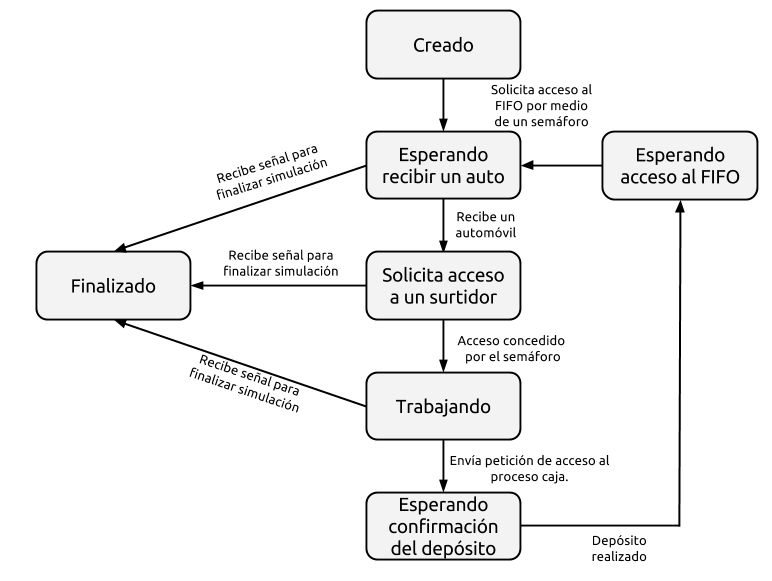
\includegraphics[scale=0.60]{FSM_Empleado.png}
	\centering
	\end{figure}

	\newpage
	\subsection{Diagrama de clase de acceso a la caja}

	\begin{figure}[h]
	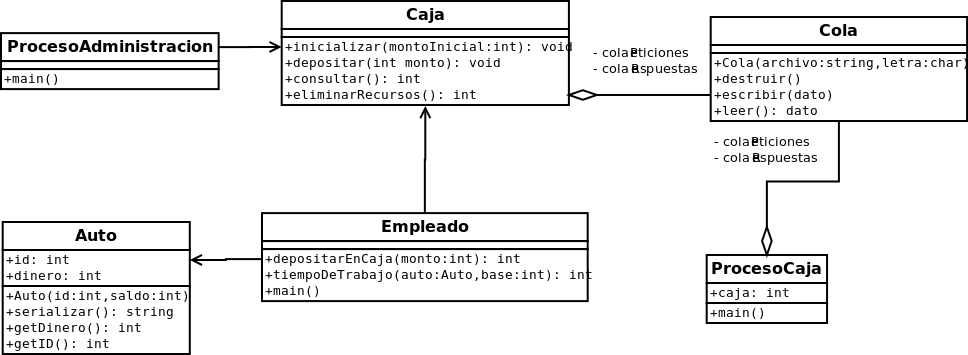
\includegraphics[angle=90,scale=0.56]{AccesoCaja2.png}
	\centering
	\end{figure}


\end{document}
